\documentclass[11pt]{article}

% Packages
\usepackage[a4paper, margin=1in]{geometry}
\usepackage{amsmath, amssymb, amsthm}
\usepackage{graphicx}
\usepackage{booktabs}
\usepackage{float}
\usepackage{hyperref}
\usepackage{setspace}
\usepackage{enumitem}
\usepackage{titling} 
\usepackage{caption}
\captionsetup{font=footnotesize, skip=3pt}

% Line spacing
\setstretch{1.15}

% ---- Title spacing control ----
\setlength{\droptitle}{-1.5cm} % moves entire title block up

\pretitle{\vspace{-0.5cm}\begin{center}\LARGE\bfseries}
\posttitle{\end{center}\vspace{-0.5cm}}

\preauthor{\begin{center}\large}
\postauthor{\end{center}\vspace{-1.5cm}}

% Title info
\title{Fisher Scoring and MCMC for GLMs}
\author{Probability and Statistics -- Final Project (Group 19)}
\date{}

% ---- spacing adjustments ----
\setlength{\abovedisplayskip}{4pt}
\setlength{\belowdisplayskip}{4pt}

% ---- custom commands ----
\newcommand{\derivstep}[1]{%
  \par\medskip\noindent #1%
}



\begin{document}

\maketitle
% GLMs and Algorithms
\section{Generalized Linear Models and Algorithms}

\subsection{Generalized Linear Models (GLM)}
A GLM extends classical linear regression to allow response variables from the exponential family. It comprises three components:
\begin{enumerate}[itemsep=1pt, topsep=4pt]
    \item Random component: $Y_i \sim f(y_i;\theta_i,\phi) = \exp\!\left\{\frac{y_i \theta_i - b(\theta_i)}{a(\phi)} + c(y_i,\phi)\right\}$
    \item Systematic component: $\eta_i = X_i^{\top} \beta$
    \item Link function: $g(\mu_i) = \eta_i$ where $\mu_i = \mathbb{E}[Y_i|X_i]$
\end{enumerate}

For canonical link functions, $ \theta_i = \eta_i = X_i^{\top} \beta$.

%------------Fisher Scoring简介-------------------------------
\subsection{Fisher Scoring Algorithm}
\subsubsection{Algorithm Description}\vspace{-4pt}
Fisher Scoring iteratively updates parameter estimates as follows::
\begin{enumerate}[itemsep=1.pt, topsep=4pt]
    \item Initialize the parameter vector $\beta_0$ (typically as a zero
    vector).
    \item For iteration $k = 0,1,2,\dots$ until convergence, update $\beta_{k+1} = \beta_k + \left[I(\beta_k)\right]^{-1} \nabla \ell(\beta_k)$,
     where $\nabla \ell(\beta_k)$ denotes the score function and $I(\beta_k)$ is the Fisher information matrix.
    \item Check convergence using a criterion such as $\lVert \nabla \ell(\beta_k) \rVert < 10^{-8}$.
\end{enumerate}


%----------------------------------推导------------------------------------------------
\subsubsection{Gradient of the Log-Likelihood}\vspace{-2pt}
The log-likelihood is
$
\ell(\beta) = \sum_{i=1}^n
\left[
\frac{y_i\theta_i - b(\theta_i)}{a(\phi)} + c(y_i,\phi)
\right].
$

\derivstep{For exponential families, }
$\mu_i = b'(\theta_i) \qquad\mathrm{Var}(Y_i\mid x_i) = b''(\theta_i)a(\phi)$\vspace{-4pt}
\[
\frac{\partial \ell(\beta)}{\partial \beta_j}
= \sum_{i=1}^n
\frac{\partial \ell_i}{\partial \theta_i}
\frac{\partial \theta_i}{\partial \mu_i}
\frac{\partial \mu_i}{\partial \eta_i}
\frac{\partial \eta_i}{\partial \beta_j}
=\sum_{i=1}^n
\frac{y_i - \mu_i}{a(\phi)}
\frac{a(\phi)}{\mathrm{Var}(Y_i \mid x_i)}
\frac{1}{g'(\mu_i)}
x_{ij}
= \sum_{i=1}^n
\frac{(y_i - \mu_i)x_{ij}}
{\mathrm{Var}(Y_i\mid x_i)\, g'(\mu_i)}.
\]
\noindent In matrix form, 
$
\nabla \ell(\beta)
= X^\top A (y - \mu)$, where $A = \mathrm{diag}\left(
\frac{1}{\mathrm{Var}(Y_i\mid x_i)g'(\mu_i)}
\right).
$

\derivstep{For canonical link function, }$\theta_i = \eta_i$, so
$
\frac{\partial \ell(\beta)}{\partial \beta_j}
= \sum_{i=1}^n
\frac{y_i - \mu_i}{a(\phi)} x_{ij}
$ or $\nabla \ell(\beta) = \frac{1}{a(\phi)} X^\top (y - \mu)$.
\derivstep{For Bernoulli and Poisson models in particular, } $a(\phi)=1$, and hence $\nabla \ell(\beta) = X^\top (y - \mu)$.
%------------信息矩阵推导-----------------------------------------
\subsubsection{Fisher Information Matrix}\vspace{-2pt}
The $(j,k)$-th element of the Fisher information matrix is defined as \vspace{-4pt}
\[
I_{jk}(\beta)
= \mathbb{E}\!\left[
\frac{\partial \ell(\beta)}{\partial \beta_j}
\frac{\partial \ell(\beta)}{\partial \beta_k}
\right]
= \mathbb{E}\!\left[
\left(
\sum_{i=1}^n
\frac{(y_i - \mu_i)x_{ij}}
{\mathrm{Var}(Y_i)\, g'(\mu_i)}
\right)
\left(
\sum_{i=1}^n
\frac{(y_i - \mu_i)x_{ik}}
{\mathrm{Var}(Y_i)\, g'(\mu_i)}
\right)
\right]
= \sum_{i=1}^n
\frac{x_{ij} x_{ik}}
{\mathrm{Var}(Y_i)\,[g'(\mu_i)]^2}
\]
In matrix form, $I(\beta) = X^\top W X,$
where $W = \mathrm{diag}(w_1,\dots,w_n),\qquad w_i = \frac{1}{\mathrm{Var}(Y_i)\,[g'(\mu_i)]^2}$


\derivstep{Logistic regression (logit link): }
$\mathrm{Var}(Y_i)=\mu_i(1-\mu_i)$ and
$g'(\mu_i)=\dfrac{1}{\mu_i(1-\mu_i)}$, so
$w_{ii}=\mu_i(1-\mu_i)$.

\derivstep{Poisson regression (log link): }
$\mathrm{Var}(Y_i)=\mu_i$ and $g'(\mu_i)=\frac1{\mu_i}$, so 
$w_{ii}=\mu_i$.

\subsubsection{Equivalence of Fisher Scoring and Newton's Method under Canonical Links}\vspace{-2pt}
Newton's method updates $\beta^{(k+1)} = \beta^{(k)} - (\nabla^2\ell(\beta^{(k)}))^{-1}\nabla\ell(\beta^{(k)})$, while Fisher Scoring replaces $-\nabla^2\ell$ by $I(\beta) = \mathbb{E}[-\nabla^2\ell(\beta)]$. 

\derivstep{Under a canonical link, }$\theta_i = x_i^T\beta$, so $\mu_i = b'(x_i^T\beta)$ and
$\nabla^2\ell(\beta) = -\sum_i \frac{b''(x_i^T\beta)}{a(\phi)} x_i x_i^T,$
which depends only on $\beta$ and $X$, not on the random data $y_i$. 

\derivstep{Hence } $\mathbb{E}[\nabla^2\ell(\beta)] = \nabla^2\ell(\beta)$, proving the two methods coincide.

%----------MCMC------------------------------------------
\subsection{MCMC - Random Walk Metropolis-Hastings (RWMH)}
\subsubsection{Algorithm Description}\vspace{-2pt}
Under the Bayesian framework, we use $p(\beta | y, X) \propto p(y | X, \beta) \;p(\beta)$ for inference. When direct sampling is infeasible, the RWMH algorithm provides a Markov chain Monte Carlo (MCMC) approach, i.e. constructs a Markov chain with stationary distribution equal to the posterior:
\begin{enumerate}[itemsep=1pt, topsep=4pt]
    \item Choose an initial
    $\beta^{(0)}$ and a symmetric proposal distribution, e.g. 
    $
    q\!\left(\beta^\ast \mid \beta^{(t)}\right)
    = \mathcal{N}\!\left(\beta^{(t)}, \Sigma\right).
    $
    \item At iteration $t+1$, draw candidate $\beta^* \sim q(\beta^* | \beta^{(t)})$.
    \item Compute the acceptance
    probability $\alpha = \min\!\left(1,\,\frac{p(\beta^\ast \mid y, X)}{p(\beta^{(t)} \mid y, X)}\right)$.
    \item Draw $u \sim \mathcal{U}(0,1)$. If $u \leq \alpha$, set $\beta^{(t+1)} = \beta^*$; otherwise $\beta^{(t+1)} = \beta^{(t)}$.
\end{enumerate}
%----------接受率推导-------------------------------------
\subsubsection{Acceptance Probability Derivation}\vspace{-2pt}

In RWMH, the proposal distribution is symmetric and satisfies $q(\beta^\ast \mid \beta^{(t)}) = q(\beta^{(t)} \mid \beta^\ast)$, so the acceptance probability simplifies to $\alpha = \min\{1, \frac{p(\beta^*|y,X)}{p(\beta^{(t)}|y,X)}\}$.
\derivstep{For numerical stability, the acceptance probability is evaluated on the
logarithmic scale. A proposal is accepted if }$\log u < \log p(\beta^\ast \mid y, X) - \log p(\beta^{(t)} \mid y, X)$.
%------------关于prior的讨论--------------------------------
\subsubsection{Discussion of the Prior Distributions Chosen}\vspace{-2pt}
For both datasets, we used independent Gaussian priors $\beta \sim \mathcal{N}(0, \sigma^2\mathbf{I})$.
\begin{enumerate}[itemsep=1pt, topsep=4pt]
  \item Weakly Informative Nature. Setting large variances ($20.0$ for \texttt{CreditCard}, 25.0 for \texttt{azcabgptca}) so the prior is weakly informative and the posterior is driven mainly by the data.
  \item Symmetry and Neutrality. Centering at zero encodes no directional preference a priori, letting the sign and magnitude of covariate effects be determined by the observed data.
\end{enumerate}

% --------------------关于non-canonical的讨论-------------------------------
\subsection{Key Differences Induced by Non-Canonical Link Functions}
\subsubsection{Loss of Equivalence Between Fisher Scoring and Newton's Method}
\[
\frac{\partial^2 \ell(\beta)}{\partial \beta_j \partial \beta_k}
= \sum_{i=1}^n 
\left[
\frac{\partial}{\partial \beta_k}(y_i - \mu_i)
\right]
\frac{x_{ij}}{\mathrm{Var}(Y_i)\, g'(\mu_i)}
+
\sum_{i=1}^n
(y_i - \mu_i)
\frac{\partial}{\partial \beta_k}
\left(
\frac{1}{\mathrm{Var}(Y_i)\, g'(\mu_i)}
\right)
x_{ij}
\]

\derivstep{Under a canonical link function, } $\frac{1}{\mathrm{Var}(Y_i)\, g'(\mu_i)} = \frac{1}{a(\phi)}$ (a constant), hence the second term vanishes. The Hessian does not depend on $y_i$ so 
$\mathbb{E}\!\left[ H(\beta) \right] = H(\beta)$ and Fisher scoring coincides with Newton's method. Under a non-canonical one, this term is no longer constant. The Hessian depends on $y_i$, so $\mathbb{E}\!\left[ H(\beta) \right] \neq H(\beta)$ and Fisher scoring and Newton's method no longer coincide.

\subsubsection{Increased Complexity of the Weight Matrix}
Under a canonical link, the diagonal weight matrix $w_i
= \frac{1}{\mathrm{Var}(Y_i)}
\left( \frac{\partial \mu_i}{\partial \eta_i} \right)^2
= \frac{b''(\theta_i)}{a(\phi)}
= \frac{\mathrm{Var}(Y_i)}{a(\phi)^2}.
$
\derivstep{Under a non-canonical link, the weight matrix becomes more complex. For instance, in the probit regression model,}
$
\mu_i = \Phi(\eta_i), \quad \mathrm{Var}(Y_i) = \mu_i(1-\mu_i) = \Phi(\eta_i)\bigl(1-\Phi(\eta_i)\bigr), \quad \frac{\partial \mu_i}{\partial \eta_i} = \phi(\eta_i)
$.
The corresponding weight is then
$
w_i
= \frac{1}{\mathrm{Var}(Y_i)}
\left( \frac{\partial \mu_i}{\partial \eta_i} \right)^2
= \frac{\phi(\eta_i)^2}{\Phi(\eta_i)\bigl(1-\Phi(\eta_i)\bigr)}.
$

% --------------------------------数据集分析---------------------------------
\section{Credit Card Dataset Analysis}
\textbf{Variable Exclusion:} We excluded \texttt{expenditure} and \texttt{share} as they represent post-approval behavior, introducing data leakage and potential reverse causality.
\derivstep{\textbf{Fisher Scoring:}
The Fisher scoring algorithm converged in 7 iterations. Convergence plots of the parameter estimates and log-likelihood values indicate stable and monotonic convergence.}

\derivstep{\textbf{MCMC (Random Walk Metropolis--Hastings):}} The trace plot for income shows stable fluctuations with no trend. The ACF decays rapidly (within 7 lags), indicating good mixing and adequate effective sample size.\vspace{-0.3cm}
\begin{figure}[H]
    \centering
    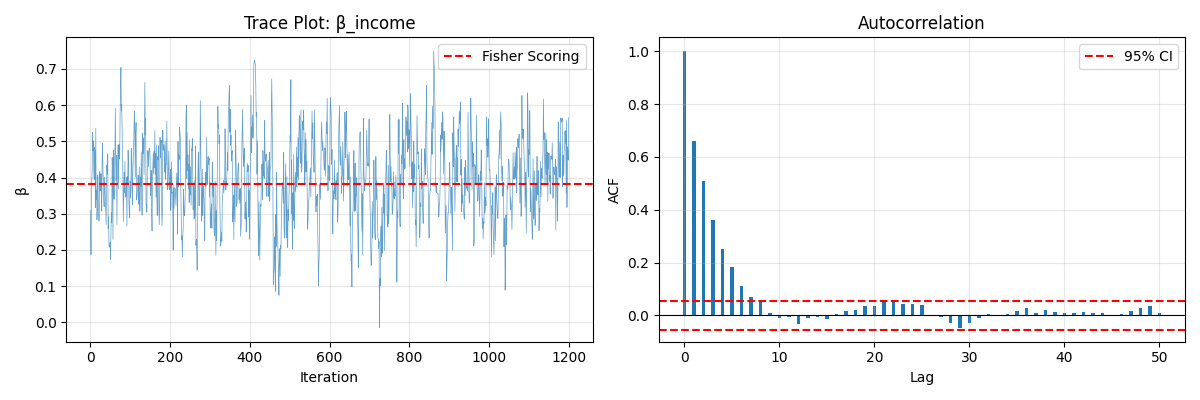
\includegraphics[width=0.95\textwidth]{mcmc_trace_acf_income.png}
    \caption{MCMC diagnostics for the income coefficient.}
    \label{fig:mcmc_diagnostics}
\end{figure}\vspace{-0.5cm}
\derivstep{\textbf{Final Discussion on the Fitted Models}}
\derivstep{Both approaches produce consistent results with similar coefficients and confidence and credible intervals overlap, confirming methodological robustness.}\vspace{-0.2cm}
\begin{table}[h!]
\centering
\footnotesize
\setlength{\tabcolsep}{3pt}
\begin{tabular}{lrrrrrrrrrr}
\toprule
Method & Intercept & reports & age & income & owner & selfemp & dependents & months & majorcards & active \\
\midrule
Fisher (Coef) & 1.2998 & -2.3565 & -0.1269 & 0.3833 & 0.4783 & -0.7573 & -0.3023 & 0.0338 & 0.1954 & 0.8342 \\
MCMC (Mean)   & 1.2889 & -2.3552 & -0.1224 & 0.3958 & 0.5138 & -0.7061 & -0.3101 & 0.0302 & 0.1921 & 0.8252 \\
MCMC (Std)    & 0.1300 & 0.1689  & 0.0959  & 0.1105 & 0.2108 & 0.2530  & 0.0840  & 0.0887 & 0.0767 & 0.1114 \\
\bottomrule
\end{tabular}
\label{tab:creditcard_results}
\end{table}\vspace{-0.5cm}
\derivstep{In the model, coefficients describe} the effect of covariates on the log-odds of credit card acceptance: positive coefficients increase the odds of approval, ceteris paribus and vice versa.
\derivstep{In our analysis, we initially used standardized covariates to identify the most influential factors by comparing the magnitudes of their coefficients}. To provide a practical interpretation for the final discussion, we back-transformed these coefficients ($\beta_{std}$) to their \textbf{original units} using the formula $\beta_{raw} = \frac{\beta_{std}}{\sigma_x}$, where $\sigma_x$ is the sample standard deviation of the original variable. This back-transformation is applied only to non-binary covariates, while binary indicators are interpreted directly. Effects are then reported in terms of the \textbf{Odds Ratio (OR)} for logistic regression or the \textbf{Incidence Rate Ratio (IRR)} for Poisson regression, computed as $\exp(\beta_{\text{raw}})$.
\derivstep{Overall, the results suggest that credit card approval is primarily driven by indicators of creditworthiness and financial reliability rather than demographic characteristics. The three most influential covariates are:}
\begin{enumerate}[itemsep=1pt, topsep=4pt]
\item \texttt{reports} (-2.3565): Each additional derogatory report reduces approval odds by 82.65\%.
\item \texttt{active} (0.8342): Each additional active credit account increases approval odds by 14.14\%.
\item \texttt{selfemp} (-0.7573): Being self-employed reduces approval odds by 53.11\% relative to employed applicants.
\end{enumerate}

%-------------------------------医院数据集分析-----------------------------
\section{azcabgptca Dataset Analysis}
\derivstep{\textbf{Fisher Scoring:}} The Fisher scoring algorithm converged in 15 iterations. Convergence diagnostics based on the log-likelihood and gradient norm show stable convergence despite mild non-monotonic behavior in the early iterations.

%-------------收敛性诊断---------------------------------------
\derivstep{\textbf{MCMC (Random Walk Metropolis--Hastings):}} The trace plot for procedure shows stable fluctuations with no trend.The ACF decays rapidly (within 10 lags), and despite minor ripples around lag 30, the overall low values indicate good convergence and sample independence.\vspace{-0.3cm}
\begin{figure}[H]
    \centering
    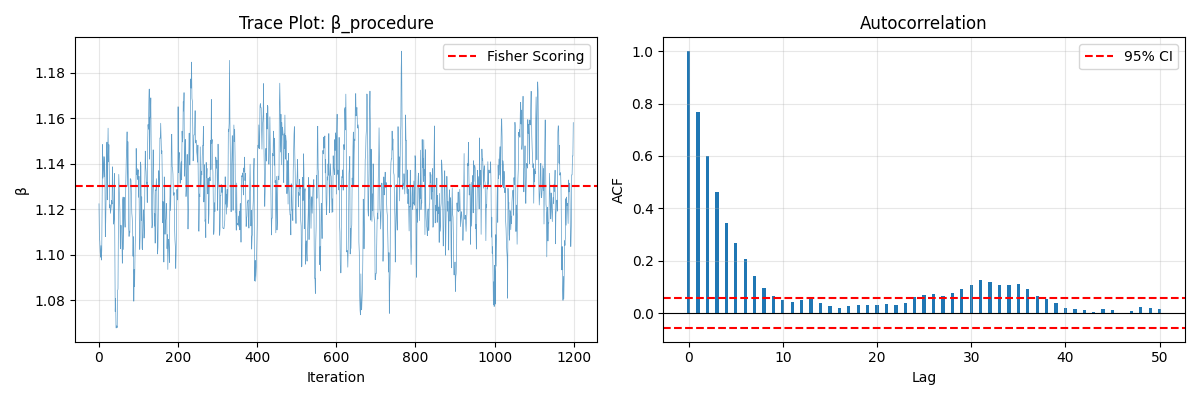
\includegraphics[width=0.95\textwidth]{mcmc_trace_acf_procedure.png}
    \caption{MCMC diagnostics for the procedure coefficient.}
    \label{fig:mcmc_procedure}\vspace{-0.5cm}
\end{figure}
%----------------------最终讨论----------------------------------------
\derivstep{\textbf{Final Discussion on the Fitted Models}}
\derivstep{Both approaches lead to consistent results regarding the determinants of hospital length of stay.}\vspace{-0.5cm}
\begin{table}[h!]
\centering
\footnotesize
\setlength{\tabcolsep}{3pt}
\renewcommand{\arraystretch}{0.9}
\begin{tabular}{lrrrrrr}
\toprule
Method & Intercept & died & procedure & age & gender & type \\
\midrule
Fisher (Coef) & 1.2821 & -0.0413 & 1.1301 & 0.0432 & -0.1061 & 0.1894 \\
MCMC (Mean)   & 1.2854 & -0.0413 & 1.1282 & 0.0433 & -0.1084 & 0.1891 \\
MCMC (Std)    & 0.0216 & 0.0081  & 0.0196 & 0.0084 & 0.0182  & 0.0178 \\
\bottomrule
\end{tabular}
\label{tab:azcabgptca_results}
\end{table}\vspace{-0.5cm}
\derivstep{In the model, coefficients describe the effect of covariates on the log of the expected hospital length of stay: positive coefficients increase the expected duration, ceteris paribus and vice versa. Overall, the results suggest that clinical factors, especially procedural invasiveness, play a dominant role in explaining hospital stay duration. The three most influential covariates are:}
\begin{enumerate}[itemsep=1pt, topsep=4pt]
\item \texttt{procedure} (1.1301): Undergoing a CABG procedure is associated with an 209.61\% increase in the expected duration of hospitalization relative to PTCA
\item \texttt{type} (0.1894): Compared to elective cases (type=0), emergency or urgent admissions (type=1) increases the expected hospital length of stay by 20.85\%.
\item \texttt{gender} (-0.1061): Male patients have an expected hospital stay that is approximately 10.06\% shorter than female ones do.
\end{enumerate}
\end{document}